%% netsoft_paper.tex
%% V1.4b
%% 2017/02/24
%% by HSNL, NTHU
%% see http://www.michaelshell.org/
%% for current contact information.


\documentclass[journal]{IEEEtran}

\usepackage{indentfirst}
\usepackage{graphicx}
\usepackage{caption}
\usepackage{subfigure}
\usepackage{enumerate}
\usepackage{epstopdf}
\usepackage{csquotes}
\usepackage[flushleft]{threeparttable}
\usepackage{hyperref}
\usepackage{url}
\usepackage{amsmath}
\usepackage[super]{nth}
\interdisplaylinepenalty=2500

\graphicspath{{figures/}}

% correct bad hyphenation here
\hyphenation{op-tical net-works semi-conduc-tor}





\begin{document}

% title
% Linebreaks \\ can be used within to get better formatting as desired.
% Do not put math or special symbols in the title.
\title{Performance Optimization of Service Chain \\for vCPE in Small Size Network \\with OpenFlow Switch}

% author names and IEEE memberships
% \author{
% \IEEEauthorblockN{
% I-Ju Liao\IEEEauthorrefmark{1},
% Chi-Hsuan Li\IEEEauthorrefmark{1},
% I-Hsien Hsu\IEEEauthorrefmark{1},
% Chia-Chi Chen\IEEEauthorrefmark{1},
% Ching-Hsuan Chen\IEEEauthorrefmark{2},
% Che-Wei Lin\IEEEauthorrefmark{2},
% Sheng-Jung Wu\IEEEauthorrefmark{1} and
% Nen-Fu Huang\IEEEauthorrefmark{1}
% }
% \IEEEauthorblockA{
% \IEEEauthorrefmark{1}
% Department of Computer Science National Tsing Hua University, Hsinchu, Taiwan\\
% }
% \IEEEauthorblockA{\IEEEauthorrefmark{2}
% Institute of Communication Engineering National Tsing Hua University, Hsinchu, Taiwan\\
% }
% }

% The paper headers
% \markboth{Journal of \LaTeX\ Class Files,~Vol.~14, No.~8, August~2015}%
% {Shell \MakeLowercase{\textit{et al.}}: Bare Demo of IEEEtran.cls for IEEE Journals}

% make the title area
\maketitle

% As a general rule, do not put math, special symbols or citations
% in the abstract or keywords.
\begin{abstract}
This Article is about a system how to optimize a service chain in SMB Network. There are many vCPE researches on Internet but a few to discuss about organization of Openflow switch and NFVs. This paper will propose a framework to optimize and manage NFVs with multi tables of Openflow switch. Most of paper talking about how to build architecture in Core Network of ISP, this paper will focus on how to use tables in SDN switches to maximum efficiency on Internet.
\end{abstract}

% Note that keywords are not normally used for peerreview papers.
\begin{IEEEkeywords}
Software defined networking, vCPE
\end{IEEEkeywords}

\IEEEpeerreviewmaketitle{}





% Introduction
% First paragraph of paper need be big Alhabet
\section{Introduction}
\IEEEPARstart{T}{his} document is a template for Microsoft Word versions 6.0 or later. If you are reading a paper or PDF version of this doconference.
By Eric





\section{Related Work}
By Eric





\section{System Description}
\subsection{Overview of Network Function}\label{ssec:desc_nfv_overview}
With the concept of SDN-enabled VNFs, SDN technology work not only for traffic steering but also as a part of network functions. In this idea, network functions have been achieved by the synergies between computer and network infrastructures, shown in Fig. \ref{fig:desc_nfv_overview}. The former is a VNF controller, mainly responsible for dealing with stateful processing. The latter is a SDN switch, used for stateless processing.

\subsubsection{Stateful Processing component (VNF controller in container)}
This component have to control the workflow, keep the state associated with the VNF, and provide interface for service providers or customers to configure and update the behavior of the stateless datapath processing component. We use SDN controller to implement the NFV controller and it’s worth noting that we use southbound APIs of SDN controller framework to handle the interface between the stateful and stateless component with OpenFlow protocol, which was originally designed for this.

\subsubsection{Stateless Processing component (SDN datapath)}
Stateless processing component, are implemented by SDN datapath resources, which is optimized for data plane traffic processing. Since SDN switch have decoupled the control plane and data plane, so it can accept the control message from the stateful processing component.

Using the advantages of this architecture, we can assign stateless or light-weight state work to the SDN switch, for example, packet filtering and packet counting, to load-off the computing resources. If we want to update our service, we just need to update the stateful component, since the stateless component just follow the command from stateful components

\begin{figure}[!t]
\centering
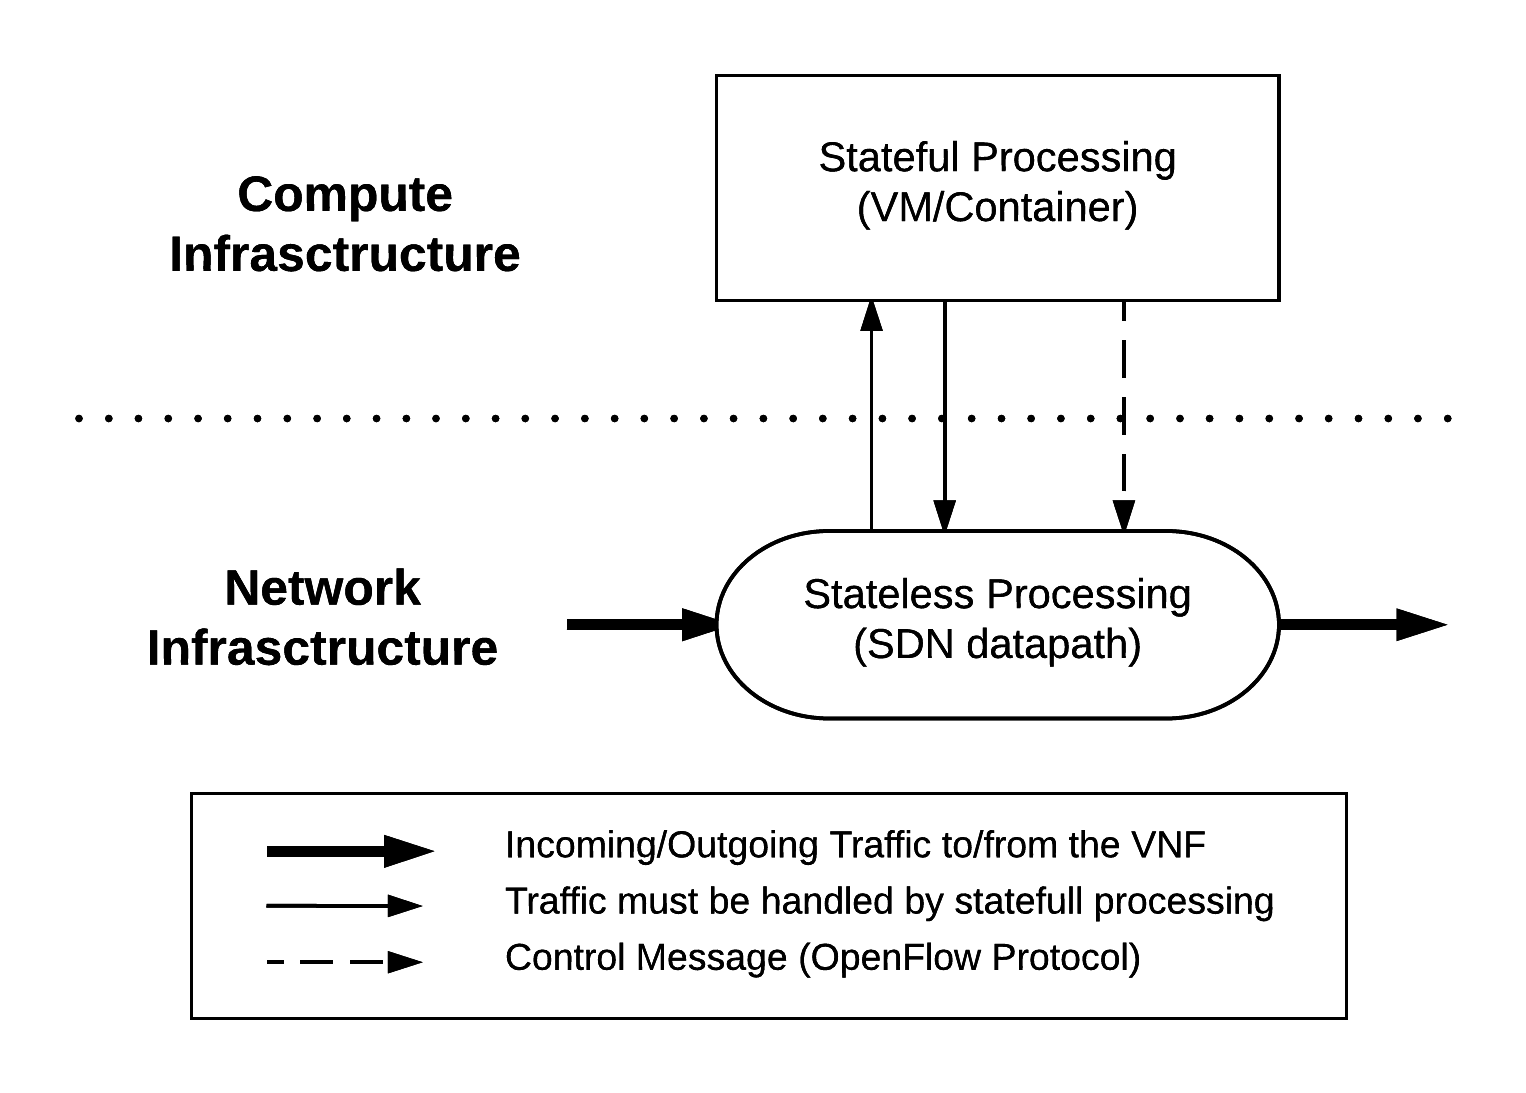
\includegraphics[width=3in]{./figures/desc_nfv_overview}
\caption{Overview of network function.}
\label{fig:desc_nfv_overview}
\end{figure}



\subsection{Service Deployment Model}
With architecture mentioned in Fig. \ref{fig:desc_nfv_overview}, we come up with a network function service deployment model. Because computing infrastructures handles the algorithm and policies, and the generic network devices only do stateless processing, the customer just need to buy a general SDN switch at their home gateway and will have a different network function service by subscribing different the NFV controller through our vCPE platform.

Fig. \ref{fig:desc_service_deployment} illustrates the service deployment model. Each green area is a local network domain of customer. At the gateway of this domain, there’s a SDN-enabled switch. The customer can subscribe to our vCPE service through our dashboard. After subscribing, the vCPE system will create a new docker container, in which running a SDN controller we developed. The customer only need to setup the gateway SDN switch to connect the SDN controller by the OpenFlow protocol, then the switch will handle these service.

\begin{figure}[!t]
\centering
\includegraphics[width=3in]{./figures/desc_service_deployment}
\caption{Service deployment model.}
\label{fig:desc_service_deployment}
\end{figure}



\subsection{Architecture of the vCPE system}
The architecture as shown in Fig. \ref{fig:desc_vcpe_framework} including of a Infrastructure Controller, Infrastructure Orchestrator, Cloud Database, VNF Controllers and VNF Orchestrator.
The Infrastructure Orchestrator, VNF Orchestrator and Cloud Database are web servers
Each component is introduced in the subsection below.

\begin{figure}[!t]
\centering
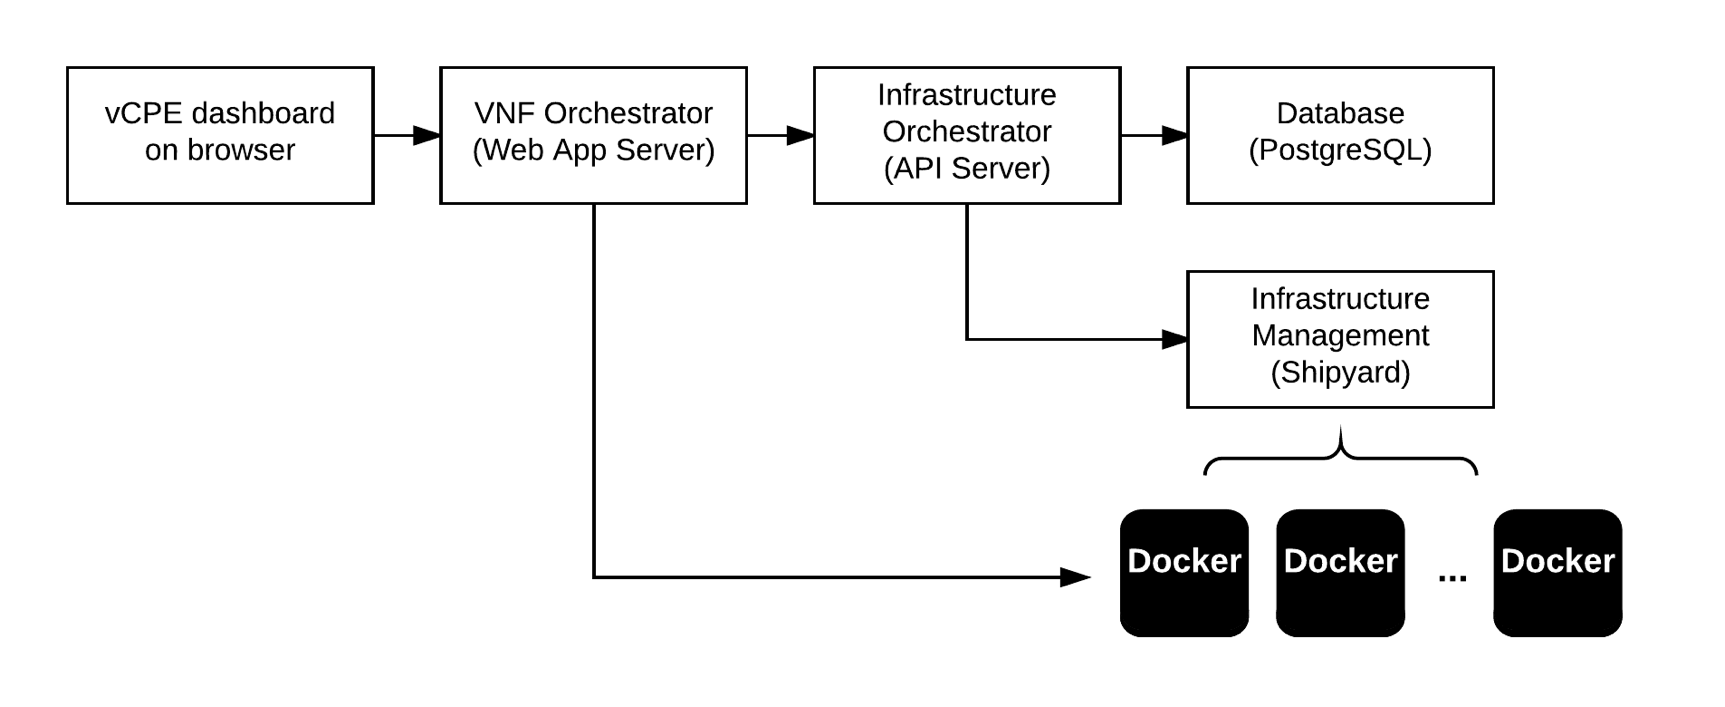
\includegraphics[width=3in]{./figures/desc_vcpe_framework}
\caption{Architecture of the vCPE framework.}
\label{fig:desc_vcpe_framework}
\end{figure}

\subsubsection{Infrastructure Controller}

The infrastructure controller is a composed Docker management server with the ability to manage the Docker resources like containers and images. The infrastructure doesn't handle the customer authentication or maintaining the state of running service, it just follows the request from the infrastructure orchestrator to create, delete, start, stop and inspect containers.

\subsubsection{Infrastructure Orchestrator}

The infrastructure orchestrator plays the key role of our system. It connecting and automating of workflows when we deploy our services. When a customer subscribes, the infrastructure orchestrator authenticates the customer first, next it will call the infrastructure controller to create a container for this customer, and update information in database afterwards. It handle the entire lifecycle of our vCPE service.

\subsubsection{Cloud Database}

The cloud database is used for restoring the of our vCPE services, which include each customer’s credential, customer’s container settings and virtual CPE service states. The cloud database is using PostgreSQL, which is a open source, easily customized and object-relational database system. Only Infrastructure Orchestrator has permissions to access cloud database.

\subsubsection{VNF Controllers}

VNF Controllers contains a SDN controller developed with ryu framework and a remote launcher module. The SDN controller does not have a remote launcher module to remotely execute a SDN controller. We built a light-weight server as a launcher module to resolve the remotely execution issue. The remote launcher module monitor the SDN controller process ID (PID) and properly kill the SDN controller process ID when on demand. When the infrastructure controller once create the container, the remote module will run up initially, waiting request from VNF Orchestrator. The details of SDN controller design will be presented at section \ref{sec:mft}.

\subsubsection{VNF Orchestrator}

The VNF Orchestrator is a Web application server hosting on Amazon Web server, being online for customer and provide a dashboard for virtual CPE and containers management and configuration.
Through the web UI provided by the VNF Orchestrator, the customers can subscribe to the desired service and without typing any command via the command line interface (CLI). After receiving the subscribing message, the VNF orchestrator will request the infrastructure orchestrator to create a new VNF controller, and then send the virtual CPE configuration to the new VNF controller. Based on configuration demands under different conditions, the network administrator is able to select any of the listed network functions on the dashboard such as Firewall, NAT, DHCP and QoS management.



\subsection{Network Functions}
The proposed vCPE service provides following network functions.

\subsubsection{Firewall}
The firewall service could filter the packets based on packet header fields, including MAC address, IP, and layer4 protocols. The network manager can add new rules or remove rules to the access control list through our vCPE GUI.

\subsubsection{NAT}
The NAT service is a network function that can remap  IP address to another one. The Source NAT (SNAT) is typically used by internal users (inside private network) to access the Internet (outside network). The network function uses the action “Set-Field”, which defined by OpenFlow protocol for rewriting packet header fields. Via vCPE GUI interface, the network manager can set up the WAN port of SDN switch, public IP, default gateway, and local network address when using this function.

\subsubsection{DHCP}
DHCP service allocates IP addresses to hosts dynamically. To implement the function, the SDN controller cope with UDP packets which use port 67 and 68. It generates DHCP offer and DHCP acknowledge to reply DHCP discovery and DHCP request received from the hosts.

\subsubsection{Forwarding}
Forwarding Service is a basic service that forward traffic to its destination and we use the Mac address learning concept to implement our forwarding function.

\subsubsection{QoS}
Quality of Service (QoS) are always used to control the traffic flows of a network and prevent the traffic to exceed the network capacity and cause traffic congestion. Therefore we implement the bandwidth management using meter which is defined within OpenFlow protocol 1.3 to set the limitation of the bandwidth.
Beside achieving network functions virtualization with SDN technology, we also make the network administrator manage and monitor a network more easily. As a result, we can offer the user the best network quality in the limited network resource without traffic congestion.
In this paper, our QoS integrates with a flow classification engine and offers the three ways of bandwidth management.

\begin{itemize}[\IEEEsetlabelwidth{Z}]
\item For a specific host.
\item For a specific application.
\end{itemize}



\subsection{Application Identifier}
Application identification is to identify each flow as an application name to enable QoS management system to do bandwidth control or distribution at application level. A flow is defined by 5-tuple (source IP, source port, destination IP, destination port, and transport layer protocol). Applications include desktop applications, native mobile applications, and web applications, such as Facebook, Skype, YouTube, Instagram, Line and WeChat. We use supervised machine learning and a method based on inspecting domain name service (DNS) responses to do flow classification. After application identification system classifies a flow as an application name, it sends the classification result to a server with database. The server stores the classification result into database, and waits for query with 5-tuple from QoS management system. The detail will be described in section \ref{sec:app_identification}.




\section{Network Function With Multiple Flow Table Management Model} \label{sec:mft}

\begin{figure*}[!t]
\centering
\includegraphics[width=6in]{./figures/mft_table_overview}
\caption{The flow table order of vCPE service.}
\label{fig:mft_table_overview}
\end{figure*}

\subsection{Multiple Flow Tables Strategy}
In subsection \ref{ssec:desc_nfv_overview}, the vCPE service design architecture have been introduced. The network functions are handled by the cooperation between SDN controller on cloud and SDN switch at the local network gateway. The controller transform the network functions to series of OpenFlow rules requests and send to SDN switch. Following the orders from controller, the SDN switch inserts rules to its flow tables, checks incoming packets against the flow entry match fields, and execute the actions in matching rules. The flow table defines all matching and corresponding processing, thus playing an important role to executive network function.

Since the flow table is a crucial component, and we find that single flow table binds us to implement our network functions. The [] also mentioned two condition for single flow table is too restrictive. The first is a single packet need to perform independent actions based on matching different fields. The second is that the packet needs two-stage processing. Involves into both situation, our network functions implemented by multiple flow tables strategy.

In multiple flow tables strategy, the most important question is: which flow table should we insert rules into? We use the network function as a demarcation, that is, SDN applications which are responsible for specific network functions will only insert rules to one specific flow table, so we can focus on the design of the network function itself. In this way, however, the order of flow table become crucial. Should we put this network function at first, or the other? The answer is about the type of match and action in the rules generated by the network function

The network functions of vCPE services including Firewall, NAT, DHCP, Forwarding and QoS. We have determined the order of each function, shown in \ref{fig:mft_table_overview}. (Notice that the flow tables are counting from zero) In the following subsections, we will introduce how to implement these network functions, which type of rules will be inserted to SDN switch, and how these rules affect our decision of the order of flow tables.



\subsection{Service Control}
Service control is about which service we want to enable or disable. To enable a service, we need to modify the table-miss rule. We always put a packet-in rule in the flow table of the last active service as a table-miss in case that there isn't any corresponding rule. To make our service chain possible, the rules of each service except the last service contains an additional action, go to next flow table, so the packets can continue to pass through all active services.

To disable a service, we not only need to modify the table-miss rule but also have to add an enforce rule. Each enforce rules has maximum priority and the action is goto next flow table. It means that packets will still pass through the disabled service's table, and the only thing they do in this flow table is ignoring other rules and go to next flow table.



\subsection{Firewall}
Firewall service is able to block traffic dynamically, and in this service, the packets will not cause any packet-in event.

On the dashboard, we can specify the blocking policies. There are 3 kinds of policies:
\begin{itemize}[\IEEEsetlabelwidth{Z}]
\item Block any traffic from a source IP or destination IP.
\item Block traffic based on known layer 4 protocols, such as SSH, HTTP, etc.
\item Block traffic to customize layer 4 ports of a host.
\end{itemize}

For different policies, the controller applies corresponding rules to the SDN switch. After the policies are set, the blocking rules will be installed immediately. Then any traffic that hit the blocking rules will be dropped. For normal traffic, they will not be affected.

As shown in Table \ref{table:fw}, all the actions of flow entries are drop. The first rule illustrates that SSH connection with source IP address 192.168.2.1 would be blocked. The second rule shows the flow entry would block the Telnet protocol.

In our multiple flow tables model, the firewall service is located in the flow table 1, since once packets are caught by the blocking rules, they doesn't need to apply any other services. The packets which match the rules will be dropped immediately, and their journey in the flow table ends here. To other no-blocked packets, they pass all blocking rules and finally match the table-miss rule, which will let the packets go on the next flow table. The action of firewall is different from other services, since in other services, no matter what actions are taken to the packets, the packets have to go to the next flow table.

% firewall example table
\begin{table*}[!t]
\caption{Firewall rules in Flow Entry}
\label{table:fw}
\centering
\begin{threeparttable}
\begin{tabular}{|l|l|l|l|l|l|}
\hline
IP proto & IP Src      & IP Dst       & L4 sport & L4 dport & Action \\ \hline
TCP      & 192.168.2.1 & *            & *        & 22       & Drop   \\ \hline
TCP      & *           & *            & *        & 23       & Drop   \\ \hline
\end{tabular}
  \begin{tablenotes}
    \item[] Symbol * represents wildcard (match any value).
  \end{tablenotes}
\end{threeparttable}
\end{table*}



\subsection{NAT}
The NAT service could allow a lot of hosts to use one public IP address to connect the network.
In order to achieve this thing, SDN controller have to set the packet header filed.  Because the SDN switch would set the field, the first packet have to go to controller. And controller would add the flow to SDN switch, after that the packet would not go to controller. It can decrease the burdens of the controller.

Below is a examples to show how the NAT service modify the IP address and port number, as shown in Fig. \ref{fig:mft_nat}. For outgoing packet, the SDN switch doesn’t have any flow entry in flow table, so the Packet-in event will be triggered at the beginning. The packet that is sent by private network host will be sent to SDN controller, and the packet header fields are modified by Set-Field action. The source IP address and source port number of outgoing packet will be modified to public IP address and remaped a new port number for NAT. For ingoing packet, the destination IP and destination port number are modified to fit private IP and port number. And then SDN controller add these flow entries to SDN switch, it can’t avoid that all the packet sent to controller.

Fig. \ref{fig:mft_nat} show the public IP address of NAT is 140.114.71.178 and a host private IP is 192.168.8.254 and port number 7878. The client sent the packet to a server with IP address 140.114.71.177 and port number 9898.

As shown in Table \ref{table:nat}, when host sent the packet to server (outgoing), the Packet-in will be trigger, and then packet to controller. The Set-Field action would modify the Source IP to public IP address of NAT is 140.114.71.178 and source port to 2000. when the server sends back to the client (ingoing), the packet header field would be modified. The destination IP address and destination port number would be modified to 192.168.8.254 and 7788.

In the single flow table framework, we have to add the two rules to SDN switch to match the outgoing and ingoing situation. At the first, we predict the NAT service to be put one the last table in the multiple flow tables framework.  Because the NAT service need to set the packet header fields and play a role of connection to the outside network. And the most important thing is that the SDN switch is according to order of table to match. We have to consider the outgoing and ingoing situations. As a result of all the above factors combined, the NAT service is located at the first and the last table in our multiple flow table framework.

\begin{figure}[!t]
\centering
\includegraphics[width=3in]{./figures/mft_nat}
\caption{The flow table order of vCPE service.}
\label{fig:mft_nat}
\end{figure}

% NAT example table
\begin{table*}[!t]
\caption{Flow entry for modifying the packet header fields of packets}
\label{table:nat}
\centering
\begin{tabular}{|l|l|l|l|l|l|}
\hline
            &IP Src          & IP Dst          & L4 src port  & L4 dst port & Action                                                                            \\ \hline
1. outgoing &192.168.8.254   &140.114.71.177   & 7878         & 9898        & \begin{tabular}[c]{@{}l@{}}IP Src $\,\to\,$ 140.114.71.178; \\ L4 src port $\,\to\,$ 2000\end{tabular} \\ \hline
2. ingoing  &140.114.71.177  &140.114.71.178   & 9898         & 2000        & \begin{tabular}[c]{@{}l@{}}IP Dst $\,\to\,$ 192.168.8.254; \\ L4 dst port $\,\to\,$ 7878\end{tabular} \\ \hline
\end{tabular}
\end{table*}



\subsection{DHCP}
DHCP service implements DHCP protocol to dynamically assign IP addresses to hosts.
DHCP operation uses UDP protocol. The clients use port 68 as the source port and 67 as the destination port.
On the contrary, the server use port 67 as the source port and 68 as the destination port.
Our system is able to handle these packets  to realize DHCP service.

The service follows these steps:
\begin{enumerate}
\item The controller adds a DHCP rule for DHCP packets when the service is enabled.
\item All packets match this DHCP rule cause packet-in.
\item The controller checks if a packet is a DHCP discovery packet. If so, the controller assigns an IP address, and generate a DHCP offer then do packet-out. If not, the controller then checks whether it's a DHCP request. If the result is positive, the controller generate a DHCP acknowledge then do packet-out.
\end{enumerate}

Our system support multiple flow table, but a specific flow table for DHCP service is not required.
The reason is that only one rule will be installed for all hosts who request for DHCP service.
When the service is disabled, the DHCP rule will be deleted,
and the packets will continue to pass through our service chain.
Following DHCP packets can reach other DHCP servers without entering our service chain
since our controller will automatically flood out broadcast packets.



\subsection{Forwarding} \label{ssec:forwarding}
In this service, when the first packet in a new connection incoming, it will cause a packet-in event because there is no corresponding rule. When controller receives the packet, it will record IP-layer information, including source IP, destination IP, input port number, source mac address and destination mac address. With the recorded information, the controller is able to install a 5-tuple forwarding rule for this connection and following packets don’t need to packet-in again. The 5-tuple is source IP, destination IP, network layer protocol, source layer 4 port, and destination layer 4 port.

In order to gather per-session statistics information, 5-tuple rules are needed. This is why we don’t add rules  based on mac address.  The controller installs a pair of dummy rules for every connection, and then request the switch to get current flow statistics every second. In this way, we can get the real-time bandwidth statistics of each connection by just subtracting the byte count from byte count of last second.



\subsection{QoS}
QoS service is mainly for traffic control and we provide three management funtion for QoS service. We will introduce these three strategy first and then discuss the flow table order of QoS service in multiple table model.

\subsubsection{Rate limitation of hosts}
When some hosts take up a lot of bandwidth of network, it will make other hosts in slow speed or make traffic congestion. To prevent this, rate limiting is used to control the rate of traffic from a host. For implementing the host rate limitation, we create a meter for desired bandwidth first and then add a flow, of which match is host’s mac address and action is the meter we just created.

The concept of this option is shown in Fig. \ref{fig:mft_qos_rate_host}. In T0, host 1 and host 2 are not limited yet. Since host 2 takes up a lot of bandwidth from network in T0~T1, the network administrator sets host 2 rate-limited under 400 Kbps. When controller receive this request, marked as (a), it will create a new meter  with meter id = 1 and bandwidth = 400 Kbps, and set the rule in the flow table with destination MAC address = HOST1 MAC and meter = 1. According to our flow table, it will limit the rate of the target host. Then the traffic from Host 2 will reduce and be limited with 400Kbps immediately. The similar situation also occurs to Host 1 in T2. The administrator chooses to set Host1 under 600 Kbps, marked as (b), and then traffic from Host 1 will be limited with 600Kbps.


\begin{figure}[!t]
\centering
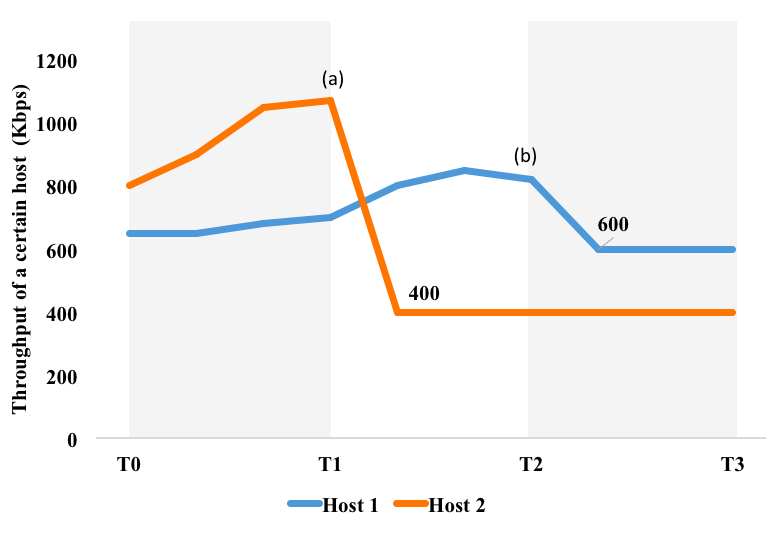
\includegraphics[width=3in]{./figures/mft_qos_rate_host}
\caption{Illustration of rate-limiting for a certain host}
\label{fig:mft_qos_rate_host}
\end{figure}


\subsubsection{Rate limitation of applications}
There are more and more network’s applications used such as online games, video streaming, conference call, etc. Therefore, there are massive traffic working in the network. Consequently, we integrate with a flow classification engine to identify the flow belongs which application is. The integration scenario will be shown as Fig. \ref{fig:class_classifying}.


In order to rate limit for a certain application, we need to gathering per-flow statistics information first. When
a connection is created, the first packet of this connection will be handled by the forwarding service and add 5-tuple rules into SDN switch, so we can get the bandwidth information of per-flow connection. (See subsection \ref{ssec:forwarding} for details). With the classified result of application identification, we can know the application type of each connection.

When network administrator request to rate limit a certain application to a certain bandwidth, we will equally distribute the bandwidth to each connection of the application. The controller set all flows belong to the same application into the same meter, and modifying the bandwidth of meter to achive our goal. For instance, if there is an application and we can find out which flows belong to this application through the flow classification engine and we want to limit this application to 1000Kbps. As Figure. \ref{fig:mft_qos_rate_app}, in T0, we know there are 3 connections belong this application and we will set the bandwidth of meter to each link with 1000/3 = 333Kbps. In T2, there are more two connections added to this application and we will reset the bandwidth of meter to each links with 1000/5 = 200Kbps. In T2, there is a connection ended by this application, we will reset the bandwidth of meter to each links with 1000/4 = 250Kbps, therefore. Whereas, the sum of bandwidth from this application is always being 1000 Kbps. That is, the bandwidth will be dynamically adjusted.

\begin{figure}[!t]
\centering
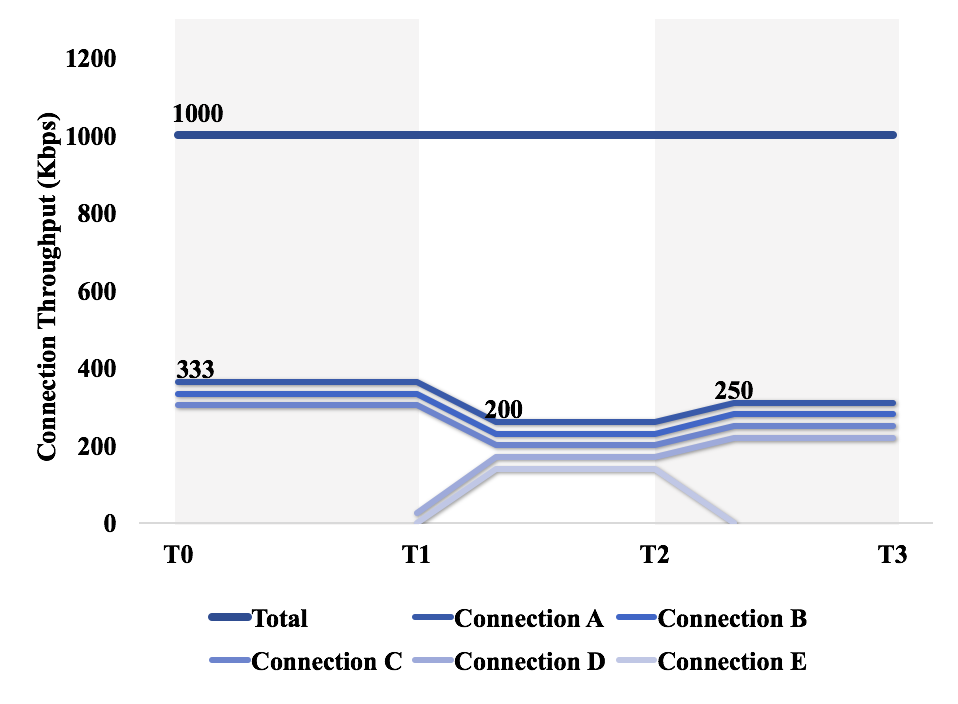
\includegraphics[width=3in]{./figures/mft_qos_rate_app}
\caption{Illustration of rate-limiting for a certain host}
\label{fig:mft_qos_rate_app}
\end{figure}

\subsubsection{The flow table order of forwarding and QoS service}
Since the location of NAT, DHCP and firewall are determined. Here we only need to decide the arrangement of QoS and forwarding.
Let's consider the scenario that we put the QoS flow table after the forwarding flow table. Plus, we have only two services enabled, forwarding and QoS, then suppose a host is not limited by QoS policies. The very first packet will not be affected in both arrangement. For the following packets, the difference can be observed. The packets which has matched the rules of the forwarding flow table will still cause packet-ins when they go to QoS flow table. This is not supposed to happen, since the host is not restrained by QoS policies and any packet-in increase the controller's load.
To reduce the burden of the controller, we put QoS flow table ahead of forwarding flow table. In this scenario, all packets that pass through QoS flow table will continue to go to forwarding flow table without matching any QoS rules. Then the packets except the very first packet will just be forwarded by forwarding service instead of causing packet-ins. Hence the controller's load will decrease. To use our system, the forwarding service is necessary, so there is no such scenario that users enable QoS and disable forwarding.






\section{Application Identification Method}\label{sec:app_identification}
In order to let QoS management system be able to control or distribute bandwidth at application level, we designed and implemented an application identification system (also called flow classification system) to judge each flow is established by what application. In other words, the system can classify each flow as an application name in real time, rather than a rough category or a transport layer protocol.
We use supervised machine learning (ML) and a method based on inspecting domain name service (DNS) responses to do flow classification. Except for DNS responses, the system only analyzes transport layer information of packets without inspecting their payload.

\subsection{Architecture of application identification system}
There are training phase (also called preparation phase) and classifying phase, their architectures are shown in Fig. \ref{fig:class_training} and Fig. \ref{fig:class_classifying} respectively. These architectures can be integrated, and do training and classifying in the same time.

\begin{figure}[!t]
\centering
\includegraphics[width=3in]{./figures/classification_training}
\caption{Architecture of our application identification system in training phase.}
\label{fig:class_training}
\end{figure}

\begin{figure}[!t]
\centering
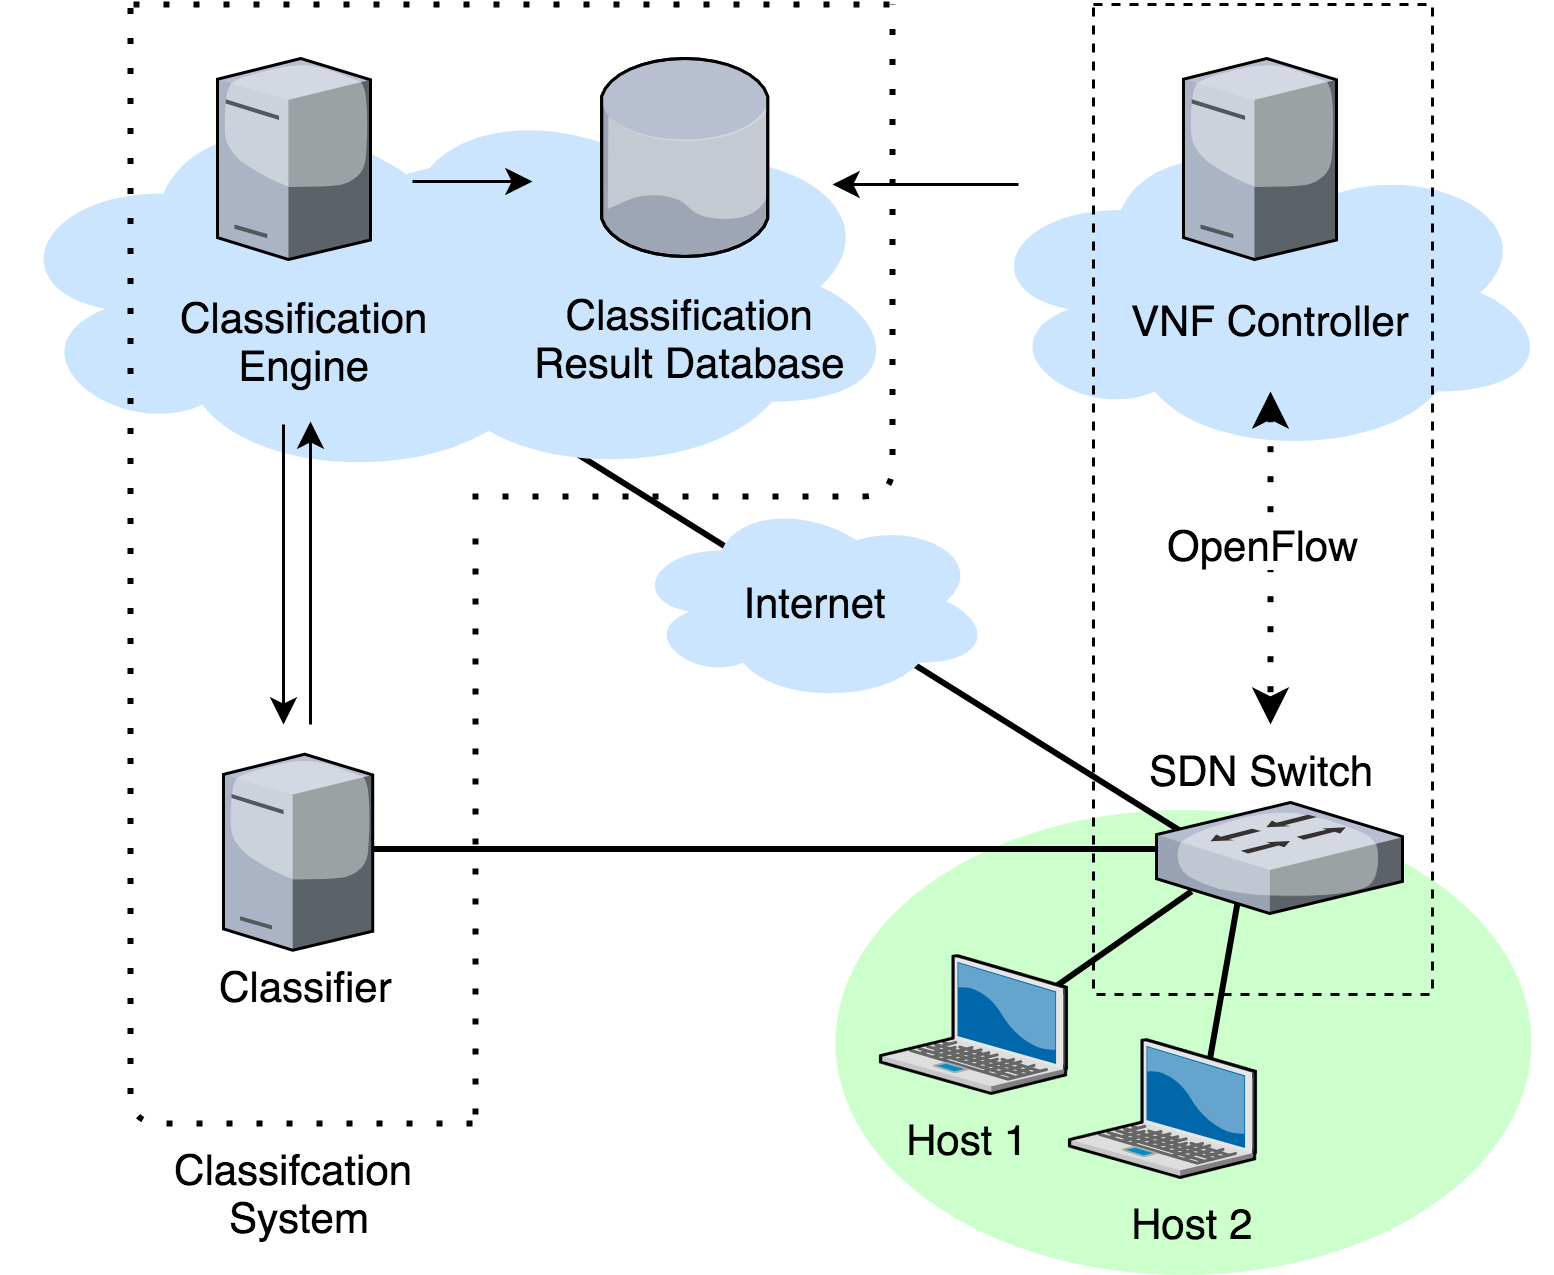
\includegraphics[width=3in]{./figures/classification_classifying}
\caption{Architecture of our application identification system in classifying phase.}
\label{fig:class_classifying}
\end{figure}



\subsection{Overall procedure of application identification}
In training phase, we generate some data needed by ML and the method based on inspecting DNS responses. In classifying phase, if a flow meet some requirement, we use the method based on inspecting DNS response to classify; otherwise, we use ML to classify.



\subsection{Procedure of Supervised ML in our system}
In training phase, the architecture is show in Fig. \ref{fig:class_training}. Flow classification engine is to build classification model by training data from Trainer, and update the model when new training data comes. Trainer is to analyze traffic from mirror port to get flow attributes. After Trainer finishes calculating flow attributes of a flow, it gets ground truth of the flow from Scanner or App Meta Server to generate training data, and sends training data to flow classification engine. App Meta Server is to store mappings of 5-tuple and ground truth from Scanner, and accept queries from Trainer. Scanner is to get mappings of 5-tuple and ground truth from OS.
In classifying phase, the architecture is shown in Fig. \ref{fig:class_classifying}. Flow classification engine is to use flow attributes from Classifier and classification model to get a classification result, and sends classification result to Classifier. Classifier is to analyze traffic from mirror port to get flow attributes. After Classifier finishes calculating flow attributes of a flow, it use flow attributes to ask flow classification engine for classification result if needed.



\subsection{Flow attributes we adopted in ML}
In ML, when system calculates flow attributes, we only use transport layer information of packets which have payload. We use Application Round (APPR) proposed by [] to analyze flow behavior. We use number of packets, packet sizes, transmission time, transmission direction, throughput, and APPR to define flow attributes. There are 69 attributes in total, as defined in our previous work



\subsection{Algorithms we adopted in ML}
We use algorithms implemented by Weka, a famous open source ML tool developed at the University of Waikato. We call Weka Java API to build classification model. We use three algorithms, namely RandomSupSpace with RandomTree [], FilterClassifier with discretization and RandomTree [], and RandomCommittee with RandomTree [].



\subsection{Procedure of a method based on inspecting DNS response in our system}
In training phase, we collect the mappings of server IP and application name. A mapping of server IP and application name means the application has ever establish connection with the server whose IP is the server IP, and the server IP has ever occurred in any DNS response we have captured.
In classifying phase, we only use those mappings which have been used by one application to classify. When system detect a flow, we check whether source IP or destination IP of the flow match any server IP of those mappings. If it matches any server IP, we regard corresponding application name as classification result; otherwise, we use flow attributes of the flow and classification model to classify.






\section{PERFORMANCE EVALUATION}
\subsection{Multiple Table Performance}

\begin{figure}[!t]
\centering
\includegraphics[width=3in]{./figures/evaluation_nat_scenario}
\caption{Multiple Table Performance Evaluation Scenario}
\label{fig:evaluation_nat_scenario}
\end{figure}

\begin{figure}[!t]
\centering
\includegraphics[width=3in]{./figures/evaluation_nat_result}
\caption{Result of Multiple Table Performance Evaluation}
\label{fig:evaluation_nat_result}
\end{figure}

The single flow table framework implementation is easier than multiple flow table framework,
but the multiple flow table framework is more flexible.
To verify the efficacy of multiple flow table vCPE framework,
this experiment use the NAT service to compare the throughput between single flow table vCPE and multiple flow table vCPE.

To begin with, an overview of the experiment environment is shown in Fig. \ref{fig:evaluation_nat_scenario}.
The NFV controller run on the Dell PowerEdge R630 Rack Server,
and the SDN switch use the Pica8 P-3290 switch.
We use the iPerf2 to generate the network traffic.
The iperf server would connect the public IP address with 140.114.71.178, and then the iperf client connect to the SDN switch, and is controlled by NFV controller.
NFV controller run the NAT service, but use the different framework that are single flow table and multiple flow table.

We use the iPerf  to generate the UDP packets and send to server from client, and set the fixed value to bandwidth at 100Mbps. These experiments would use diffrent payload sizes to inspect their performances.
As shown in Fig. \ref{fig:evaluation_nat_result}, the throughput value show that the performances of large packets such as 1024 bytes and 1470 bytes is better than small packets. Because the NAT service need to set the packet header field and small payload size would send more packets to server at the same time, the performance of larger packets is well. We can see that the throughput value of multiple table framework is close to single table framework. So we can realize the multiple table framework is more flexible than single table framework, and the performance is close to each other, which shown as Fig. \ref{fig:evaluation_nat_result}.



\subsection{Accuracy of Application Identification }
\subsubsection{Testing data set}
Testing data set are mappings of flow attributes and ground truth (also called rules). This testing data set were generated by our system in our lab in National Tsing Hua University in Taiwan in 2016. We manually operated applications to generate traffic. After the system generated rules, it exported them into a file, because we wanted to do 10-fold cross validation on the testing data set. There are 14659 rules in total, and there are 137 applications if we view each platform version of an application as one application.

\subsubsection{Validation method}
Although the system can do online training and classifying, we do offline training and classifying, shown as Fig. \ref{fig:evaluation_classification}. More specifically, when we did online training to analyze traffic, get ground truth, and export the rules into a file. We do 10-fold cross validation on the rules. There are 10 rounds in 10-fold cross validation. Each round, we split testing data set into training dataset and classifying dataset.

\begin{figure}[!t]
\centering
\includegraphics[width=3in]{./figures/evaluation_classification}
\caption{Result of Multiple Table Performance Evaluation}
\label{fig:evaluation_classification}
\end{figure}

\subsubsection{Mapping of category names}
We do name mapping on training dataset before we use training data set to build classification model, and do name mapping on classifying data set before we use classifying data set to calculate accuracy. The main reason is that some application have different ground truth in different operating system.

\subsubsection{Accuracy matrices}
To evaluate accuracy, we used precision, recall and F-measure (also called F1 score), as shown in Eq. (1), Eq. (2), and Eq. (3) []. In each round in 10-fold cross validation, we calculate precision and recall of each category to calculate F1 score of each category. After ten rounds, we calculate average

\begin{equation}
\label{eqn_1}
Precision = \dfrac{True\ positive}{True\ positive\ +\ False\ positive}
\end{equation}

\begin{equation}
\label{eqn_2}
Recall = \dfrac{True\ positive}{True\ positive\ +\ False\ negative}
\end{equation}

\begin{equation}
\label{eqn_3}
F1\ score = \dfrac{2\times Precision\times Recall}{Precsion + Recall}
\end{equation}

\subsubsection{Accuracy analysis}



\subsection{QoS Evaluation Limit Host bandwidth}

We choose a way to verify our function is downloading the file in that it is a situation always takes up the network recourse in real world. We decide to download the image of Ubuntu 14.04 which is about 1GB size.

As shown in Fig. \ref{fig:qos_limit_host}, The NFV controller run on the Dell PowerEdge R630 Rack Server, and would excute the QoS service. And the OpenFlow-enable switch use the the Edge-Core AS5712-54X switch that operating system is PicOS TM r2.6.

We used a desktop computer to be the experimental host and record the bandwidth in every 2 seconds. In the beginning, we start downloading the file without limiting and the rate is between 190000 Kbps to 410000 Kbps.
At \nth{10} seconds, we wanted to limit this host’s bandwidth to 1024Kbps and we added the rule the destination MAC address is matching this desktop computer with a meter of 1024Kbps. Then we can find out the bandwidth from this host is decrease and be limited to about 1024Kbps immediately.

At \nth{36} seconds, we cancel the limit to this host. That is, removing the meter field from the rule in the flow table. Obviously, we also observed the bandwidth of download from this host is rising rapidly and without limiting.

\begin{figure}[!t]
\centering
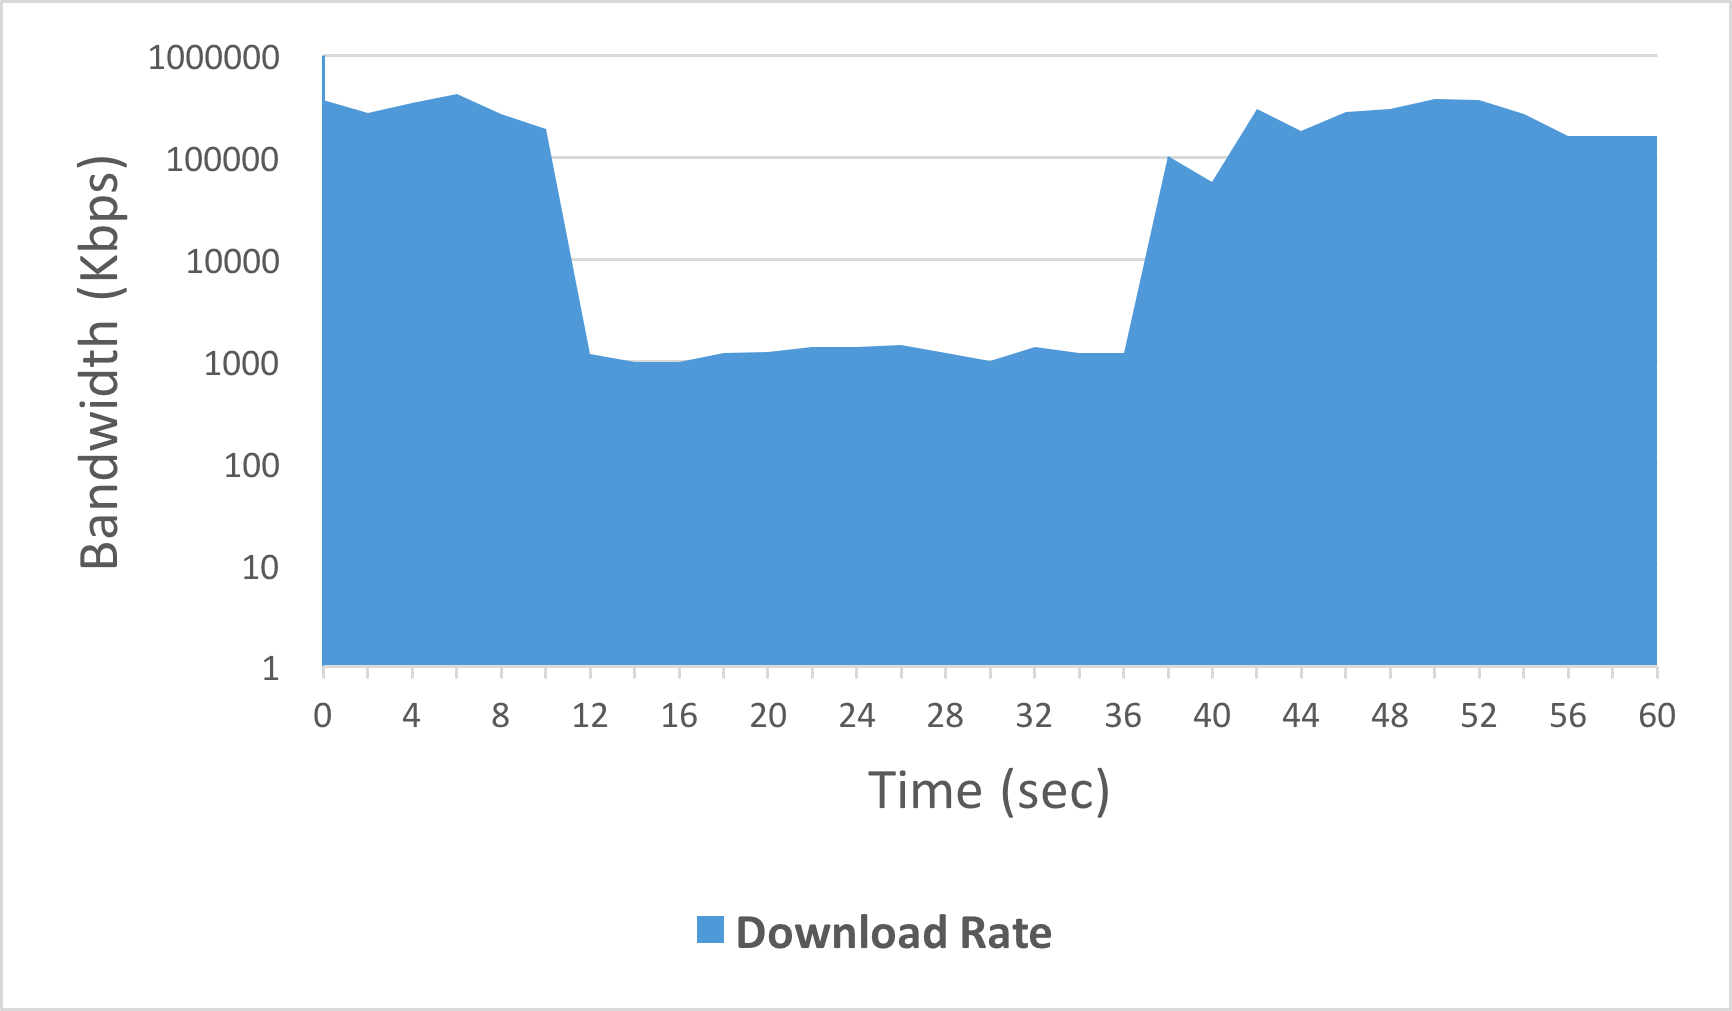
\includegraphics[width=3in]{./figures/qos_limit_host}
\caption{Limit the download rate to a host.}
\label{fig:qos_limit_host}
\end{figure}

\begin{figure}[!t]
\centering
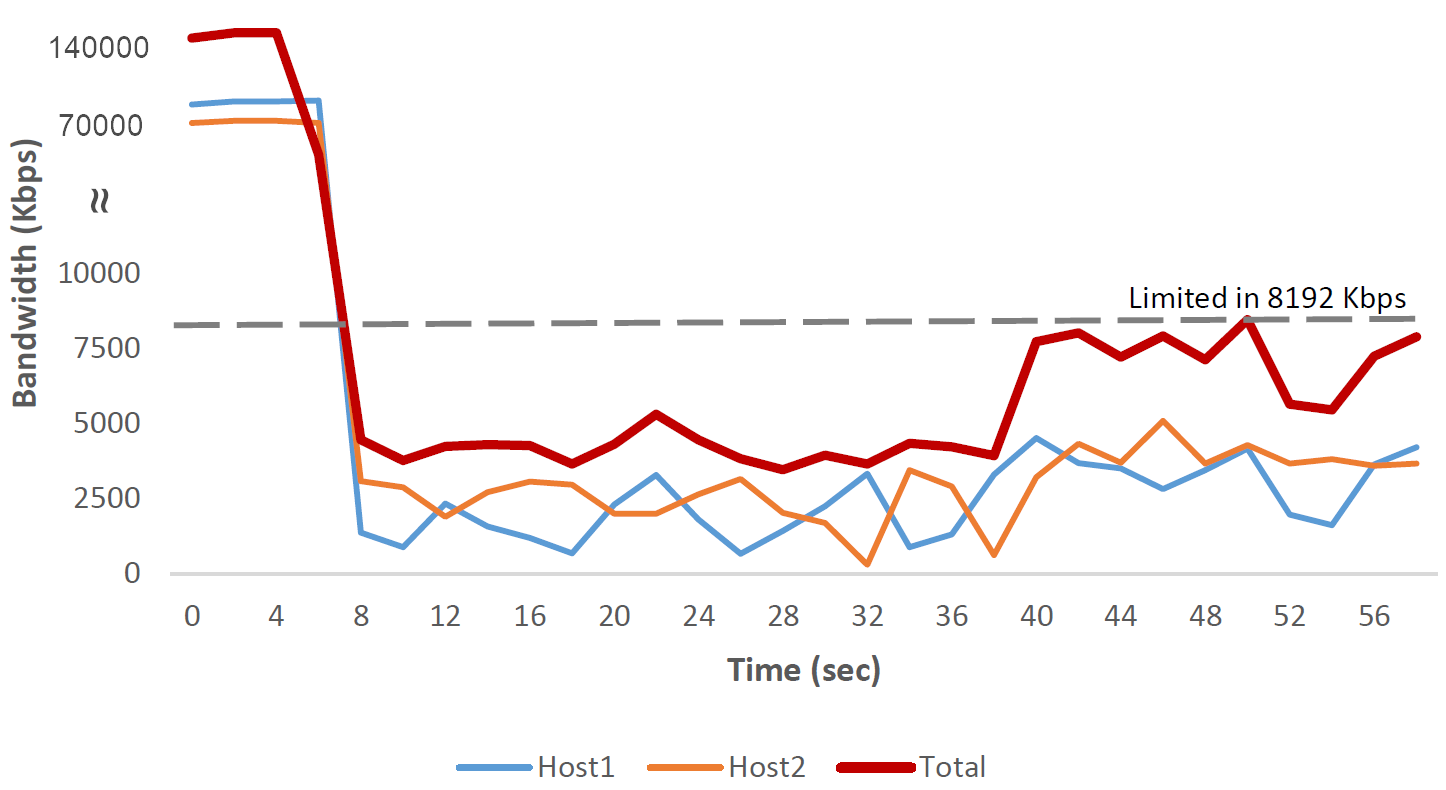
\includegraphics[width=3in]{./figures/mft_qos_rate_domain_app}
\caption{Limit the Youtube rate to a network domain.}
\label{fig:mft_qos_rate_domain_app}
\end{figure}

\subsection{QoS Evaluation Limit application bandwidth}

There are a lot of people using the streaming applications nowadays and those applications always take up an amount of network’s source. We integrated with application identification to classify each flow belongs what the application is, consequently.
We choose YouTube to verify our limitation function of applications and there are 3 Hosts (Host 1, Host 2 and Host 3) in the same network domain. Then we will limit the Youtube’s bandwidth of this network domain, that is, the sum of bandwidth from Youtube of Host 1, Host 2 and Host 3.
As shown in Figure.? In the beginning without limitation, the total bandwidth of this network is about 3000 Kbps to 4000 Kbps. At \nth{8} seconds, we limited the total bandwidth from Youtube to 2048 Kbps in this network domain. Therefore, we can find out the total traffic of Youtube from this network domain is reducing immediately. Clearly, the total traffic from Youtube will not exceed the limited bandwidth (2048Kbps) since we limited the Youtube to this network domain.
When using our limitation function of application, we can guarantee the traffic of this network domain will not over the network capacity and prevent the traffic congestion in short.

\section{Conclusion and future works}
(Eric)



\newpage
\bibliographystyle{ieeetr}
\bibliography{paper}

\end{document}
